%%This is a very basic article template.
%%There is just one section and two subsections.
\documentclass[a4paper]{article}
\usepackage[pdftex]{graphicx}
\usepackage{parskip}
\usepackage{hyperref}
\usepackage[all]{hypcap}
\usepackage{amsmath}
\usepackage{amsfonts}
\usepackage{enumitem}
\usepackage{pgfplots}
\usepackage{adjustbox}
\pgfplotsset{width=10cm,compat=1.9}
\title{Habib University \\ CS 451  - Computational Intelligence\\ Spring 2021 \\ Optimisation  and Swarm Intelligence\\Assignment  - 02}

\author{Syed Muhammad Fasih Hussain (sh05204) \\Munawwar Anwar Adam (ma04289)}
\date{\today}
\newcommand{\mat}[1]{\boldsymbol { \mathsf{#1}} }

\begin{document}
\setlength{\parskip}{10pt}
\setlength{\parindent}{0pt}
\DeclareGraphicsExtensions{.pdf,.png,.gif,.jpg}
\maketitle

\section*{Introduction}
Ant Colony Optimization (ACO) is a well-known metaheuristic in which a colony of articial ants cooperates in exploring good solutions to a combinatorial
optimisation problem. In this report, an ACO algorithim is presented for the graph coloring problem.
\section*{Problem Definition}
Let $G = (V,E)$ be an undirected graph where $V$ is the set of vertices and $E$ is the set of edges.
A $q-$coloring of G is a mapping $c\colon V \mapsto \{1,2,3,\cdots,q\}$ that assigns colors to vertices. 
The coloring is feasible if no two adjacent vertices have the same color i.e $\forall \{u,v\} \in E\colon c(u) \neq c(v)$, otherwise conflicts happen. An optimal coloring of G
is a feasible coloring with smallest number of colors. This minimum number of colors $q$ for which a feasible $q-$coloring exsists is called the chromatic number of $G$
and is denoted by $\chi(G)$. Given a graph $G$,the graph coloring problem is to find an optimal coloring. 

\section*{ANTCOL Algorithm for Graph colouring}
In ANTCOL a colony of articial ants iteratively colors a specific graph, at each iteration, initially, ants produce feasible
colorings by considering pheromone  trails and heuristic information, and afterwards pheromone trails are updated according to the quality of colorings. The
quality of colorings are measured using the following evaluation function\footnote{For presenting results in this report, f(s) = q(s).},
\begin{equation}
    f(s) = \frac{1}{q(s)}
\end{equation}
where $q(s)$ denotes the number of colors are applied in coloring $s$.\\

Pheromone trails are related to pairs of nonadjacent vertices.Therefore, each pair of nonadjacent vertices $\{v_i,v_j\}$ has an associated pheromone trail
$\tau _{ij}$ that represents the colony experience of colorings in which the two mentioned vertices have the same color i.e. belong to the same class of color. \\

There are multiple constructive methods that are used for graph coloring but here we are just focusing on ANTRLF. In ANTRLF,there exsits several stages, at stage k the artificial ant constructs color class $C_k$, and stage k also consists of several steps, at each step the artificial ant determines which uncolored vertices are to be added the color class $C_k$. Let W be the set of uncolored vertices that can be added to $C_k$, and B be the set 
of uncolored vertices which are not allowed to be added in $C_k$. In order to choose the uncolored vertex $v_i$,ANTRLF can use three diffrent peices of heuristic information as follows
\begin{equation}
\eta_{ik} = deg_{B}(v_i)  
\label{eqn:strat1}  
\end{equation}
\begin{equation}
    \eta_{ik} = deg_{B \cup W}(v_i)
    \label{eqn:strat2}    
\end{equation}

\begin{equation}
    \eta_{ik} = \mid W \mid  - deg_{w}(v_i)
    \label{eqn:strat3}    
\end{equation}
However,at the beginning of stage $k$,there are no vertices in $B$, so the following two strategies are applied to the first vertex to $C_k$
\begin{itemize}
    \item Randomly selecting an uncolored vertex from $W$
    \item Selecting vertex $v_i$ with maximum $deg_{w} (v_i)$
\end{itemize}

Pheromone trails are initially set to 1 and at the end of each iteration they are updated by considering the following rule,
\begin{equation}
    \tau_{ij} = (1 -\rho) \tau_{ij} + \sum_{s \in S_{ij}} \frac{1}{q(s)}
\end{equation}
where $q(s)$ represents the number of colors applied to coloring $s$ and $\rho$ denontes the pheromone evaporation rate. $S_{ij}$ is the subset of colorings 
in which the two vertices $v_{i}$ and $v_{j}$ belong to the same color class. In order to choose an uncolored vertex $v_i$ to be added to the color class $C_k$ , pheromone trail
is defined as follows 
\begin{equation}
    \tau_{ik} = \frac{\sum_{j \in C_{k}} \tau_{ij}}{\mid C_k \mid}
\end{equation}
$\tau_{ik}$  contains all the pheromone trails between the vertex $v_{i}$ and so far added vertices in color class $C_k$. Consequently at each step of stage $k$, the probabilistic 
decision rule determines which uncolored vertex $v_i \in W$ is to be added to the color class $C_k$ is defined as follows
\begin{equation}
    p_{ik} = 
    \begin{cases}
        \frac{\tau_{{ij}^{\alpha}} \eta_{{ij}^{\beta} } }{\sum_{j \in W} \tau_{{ij}^{\alpha}} \eta_{{ij}^{\beta}}} & v_i \in W \\
        0 & v_i \notin W
    \end{cases}
\end{equation}
where $p_{ik}$ is the probability of selecting vertex $v_{i}$. Stage $k$ continues while $W$ remains nonempty.

\section*{Computational Results}
The parameter value for ANTLRF are $\alpha = 2 , \beta = 2 $ and $\rho = 0.5$. The colony size is set to 100 ants and termination condition is defined as the
number of iterations exceeds 50. ANTRLF was applied on the gcol1 dataset and the optimal coloring $s$ used 16 colors.   There 6 diffrent strategies that are obtainaible 
in ANTRLF via combining heuristic information strategies and the strategy to the add the first vertex $v_i$ to the color class $C_k$. The experimental results determined the 
selection of \ref{eqn:strat2} and ``Randomly selecting an uncolored vertex from W '' as the best strategy. The results obtained are summarised in the table which are then followed by the graphs 
for each combination.

\begin{center}
    \begin{tabular}{|l|l|l|}
    \hline
    Combination & Number of Colors Used & Average   Number of Colors used \\ \hline
    1           & 16                    & 17.923                          \\ \hline
    2           & 16                    & 17.481                          \\ \hline
    3           & 16                    & 17.974                          \\ \hline
    4           & 18                    & 19.978                          \\ \hline
    5           & 18                    & 19.365                          \\ \hline
    6           & 17                    & 19.32                           \\ \hline
    \end{tabular}
\end{center}

From the results presented in the table, we can see that values obtained for average number of colors used were similar regardless of what strategy was choosen to add vertex $v_i$ to the color class $C_k$. On the other hand, choosing which strategy to select
when adding the first vertex $v_i$ to the color class $C_k$ had a significant impact on the results that were obtained. The strategy of randomly selected an uncolored vertex from W performed better than selecting vertex $v_i$ which has the maximum degree in W.
Intitutively, this makes sense as randomization allows the search to escape the local optima, thereby increasing the diversity of the solutions obtained.





\begin{center}
\begin{figure}[h]
\centering
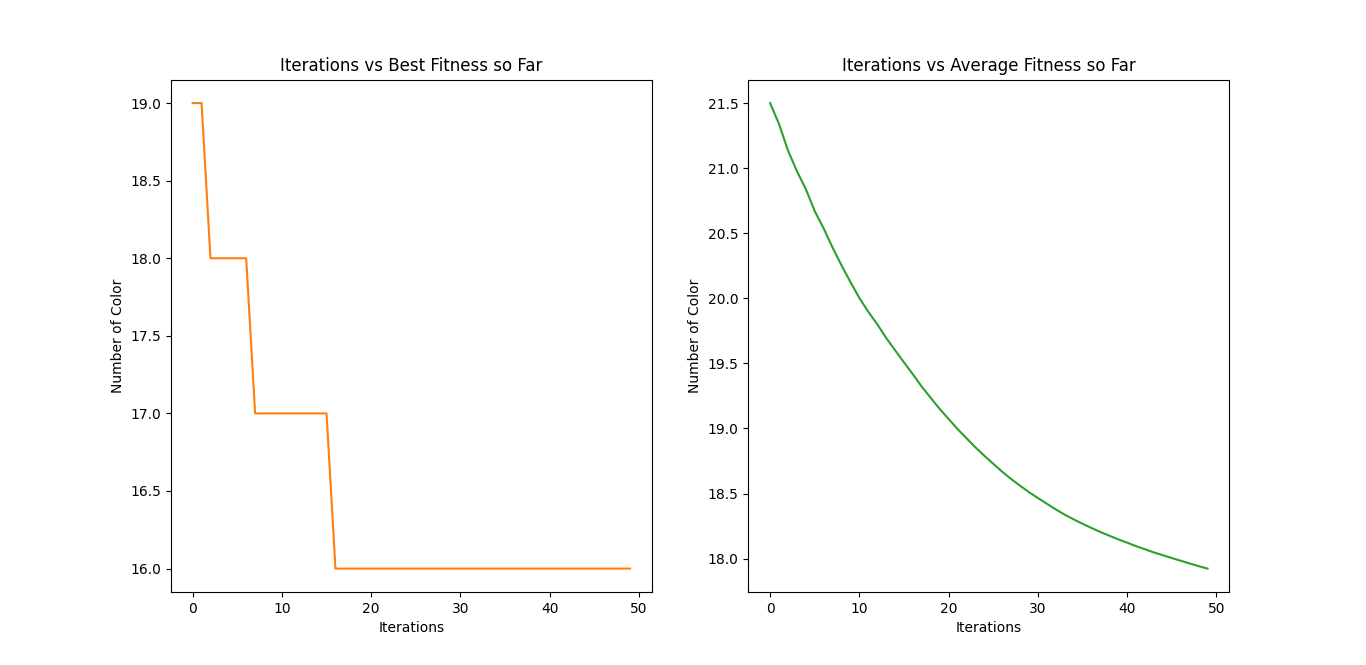
\includegraphics[width=12cm]{Figures/fig1.png}
\caption{\ref{eqn:strat1} and Randomly selecting an uncolored vertex from W.}
\label{fig:figure1}
\end{figure}
\end{center}

\newpage
\begin{center}
\begin{figure}[h]
\centering
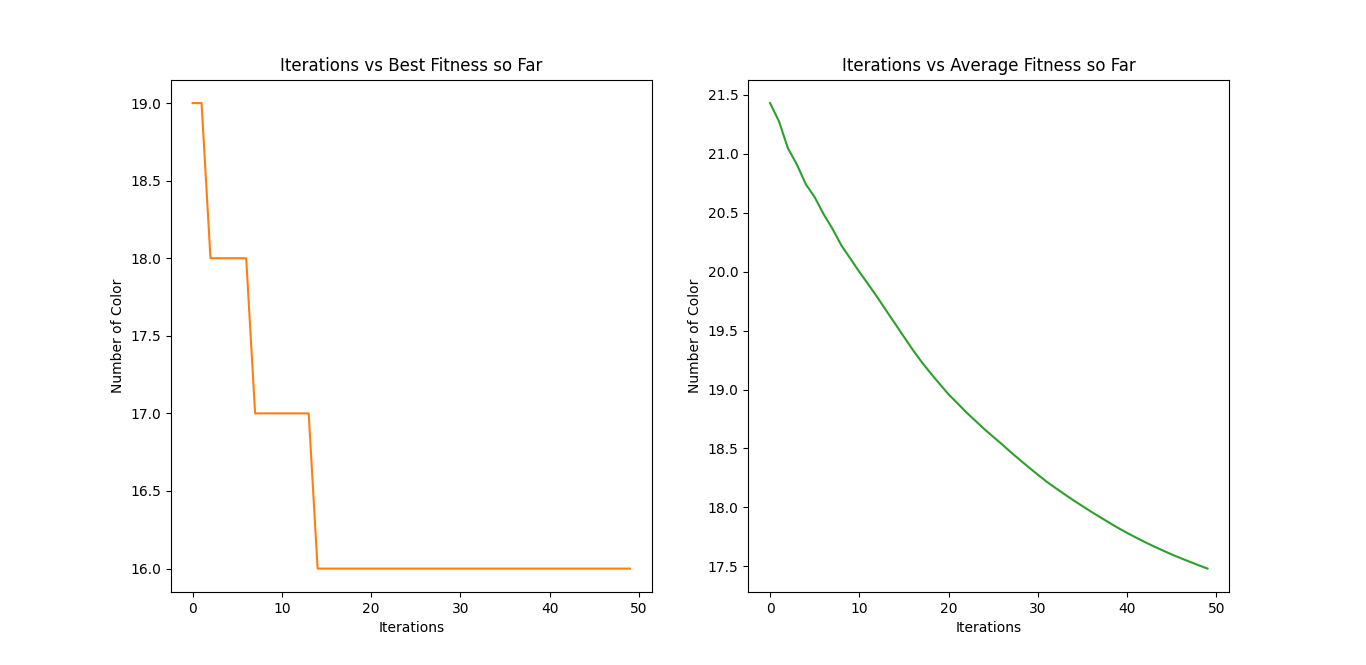
\includegraphics[width=12cm]{Figures/fig2.png}
\caption{\ref{eqn:strat2} and Randomly selecting an uncolored vertex from W.}
\label{fig:figure2}
\end{figure}
\end{center}

    
\begin{center}
\begin{figure}[h]
\centering
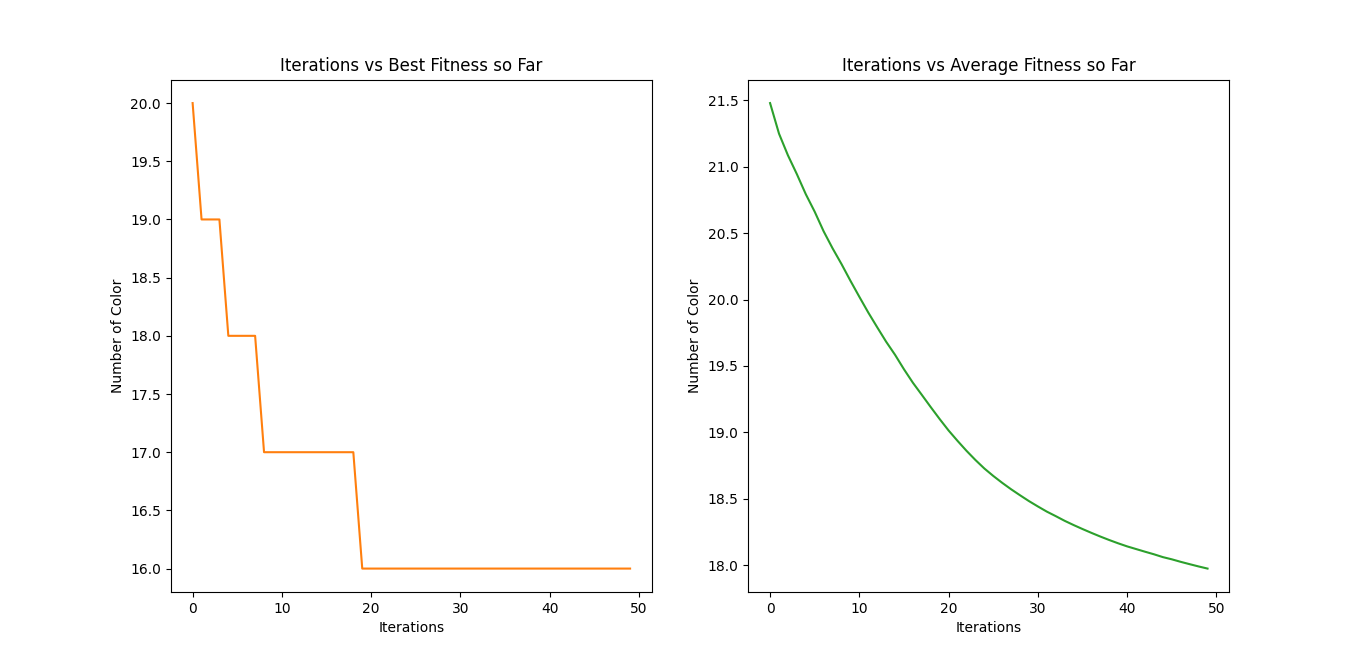
\includegraphics[width=12cm]{Figures/fig3.png}
\caption{\ref{eqn:strat3} and Randomly selecting an uncolored vertex from W.}
\end{figure}
\end{center}

    
\newpage
\begin{center}
\begin{figure}[h]
\centering
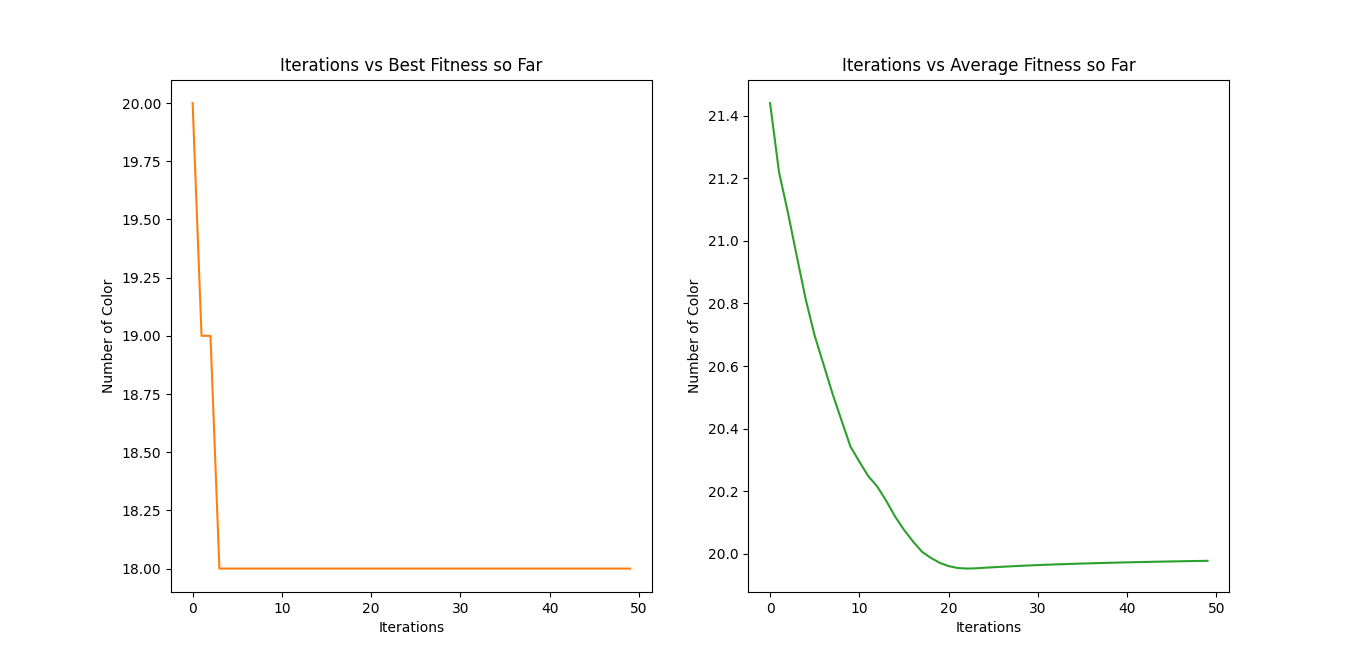
\includegraphics[width=12cm]{Figures/fig4.png}
\caption{\ref{eqn:strat1} and selecting uncolored vertex from W with maximum degree}
\end{figure}
\end{center}

    
    
\begin{center}
\begin{figure}[h]
\centering
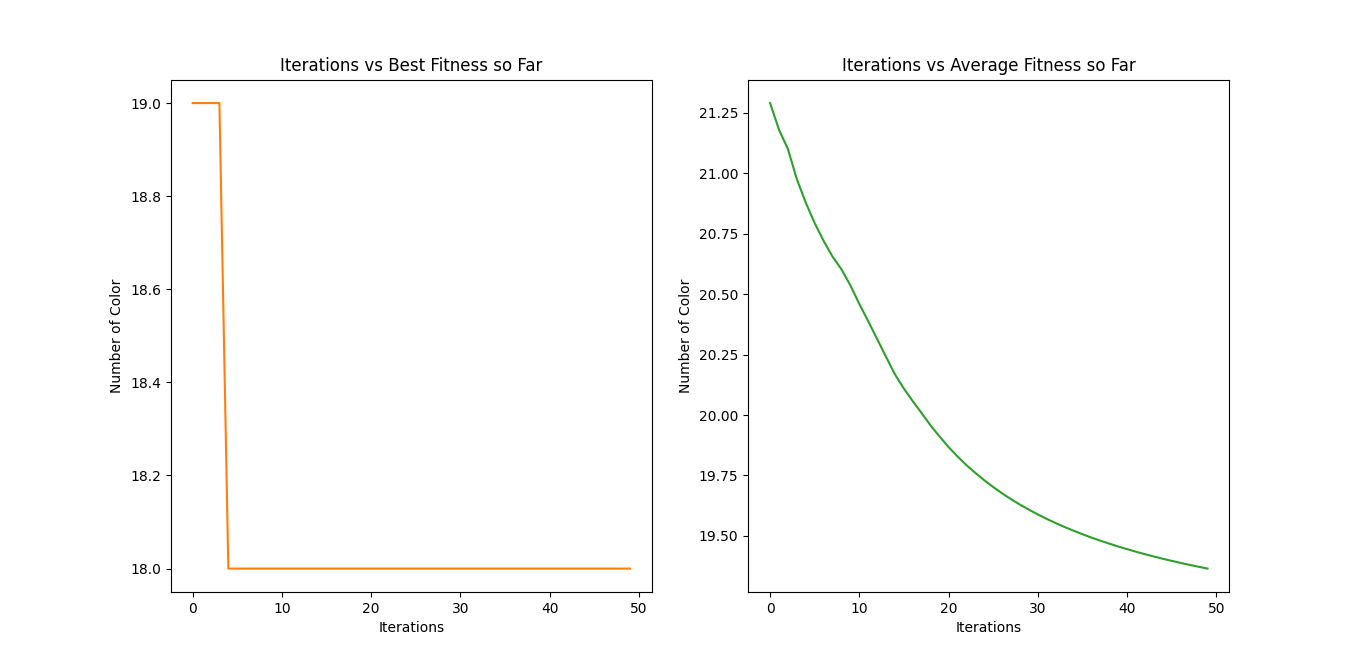
\includegraphics[width=12cm]{Figures/fig5.png}
\caption{\ref{eqn:strat2} and selecting uncolored vertex from W with maximum degree}
\end{figure}
\end{center}
    

\newpage 
\begin{center}
\begin{figure}[h]
\centering
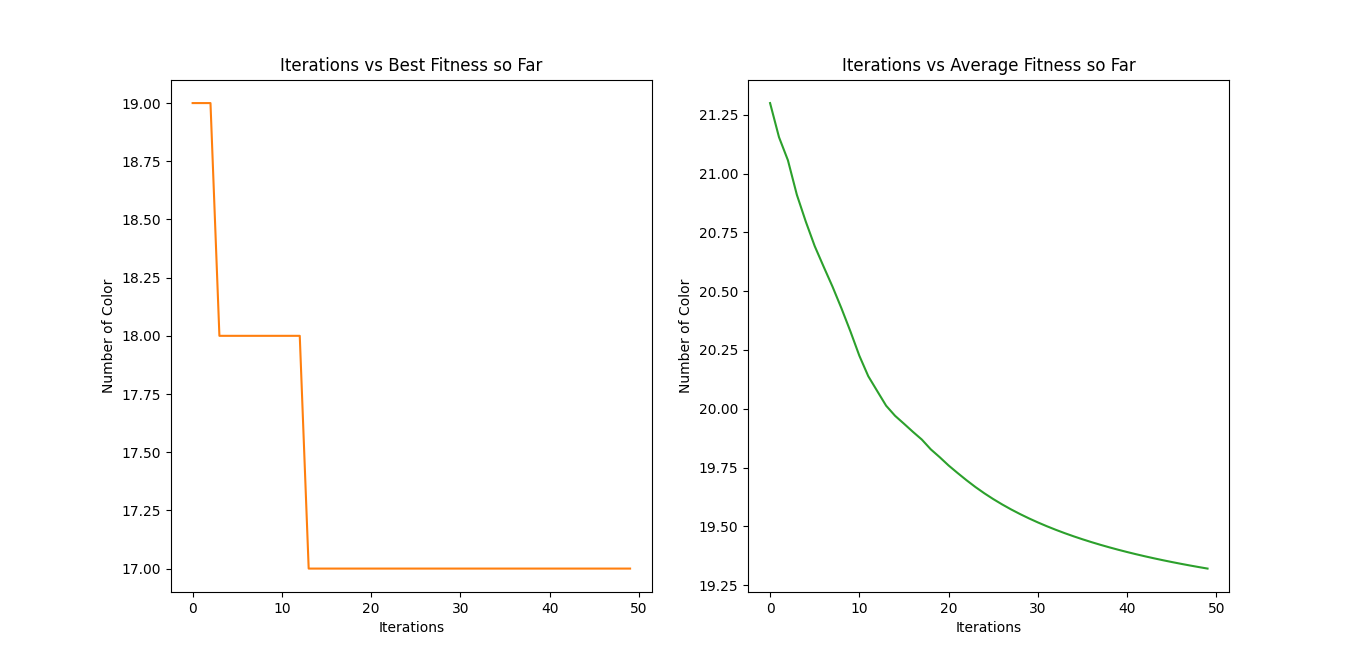
\includegraphics[width=12cm]{Figures/fig6.png}
\caption{\ref{eqn:strat3} and Randomly selecting an uncolored vertex from W.}
\end{figure}
\end{center}
    

\section*{Adjusment of the Parameters}
Various test were performed in order to obtain appropriate values of the parameters governing the search in the ANTLRF algorithim. 
The results obtained were compared with graph in \ref{fig:figure2} to determine the effacy of the changes made. When adjusting the values of diffrent parameters,
the value of other parameters was kept constant. The results are summarised in the following table. \footnote{Since this a minimisation problem, we want the value of fitness to decrease.}

\begin{center}
\begin{adjustbox}{width=1\textwidth}
\begin{tabular}{|l|l|l|l|l|l|}
\hline
Parameter & Value & Best fitness so far & Average fitness so far & Change in Best Fitness so Far. & Change in Average Fitness so Far \\ \hline
$\alpha$     & 1   & 18 & 20.735 & 2  & 3.254  \\ \hline
$\beta$      & 2   & 16 & 17.632 & 0  & 0.151  \\ \hline
$\rho$       & 0.1 & 16 & 19.402 & 0  & 1.921  \\ \hline
$N_{cycles}$ & 100 & 15 & 16.718 & -1 & -0.763 \\ \hline
$N_{ants}$   & 300 & 16 & 17.101 & 0  & -0.38  \\ \hline
$Q$          & 10  & 16 & 17.938 & 0  & 0.457  \\ \hline
\end{tabular}
\end{adjustbox}
\end{center}

\begin{center}
    \begin{figure}[h]
    \centering
    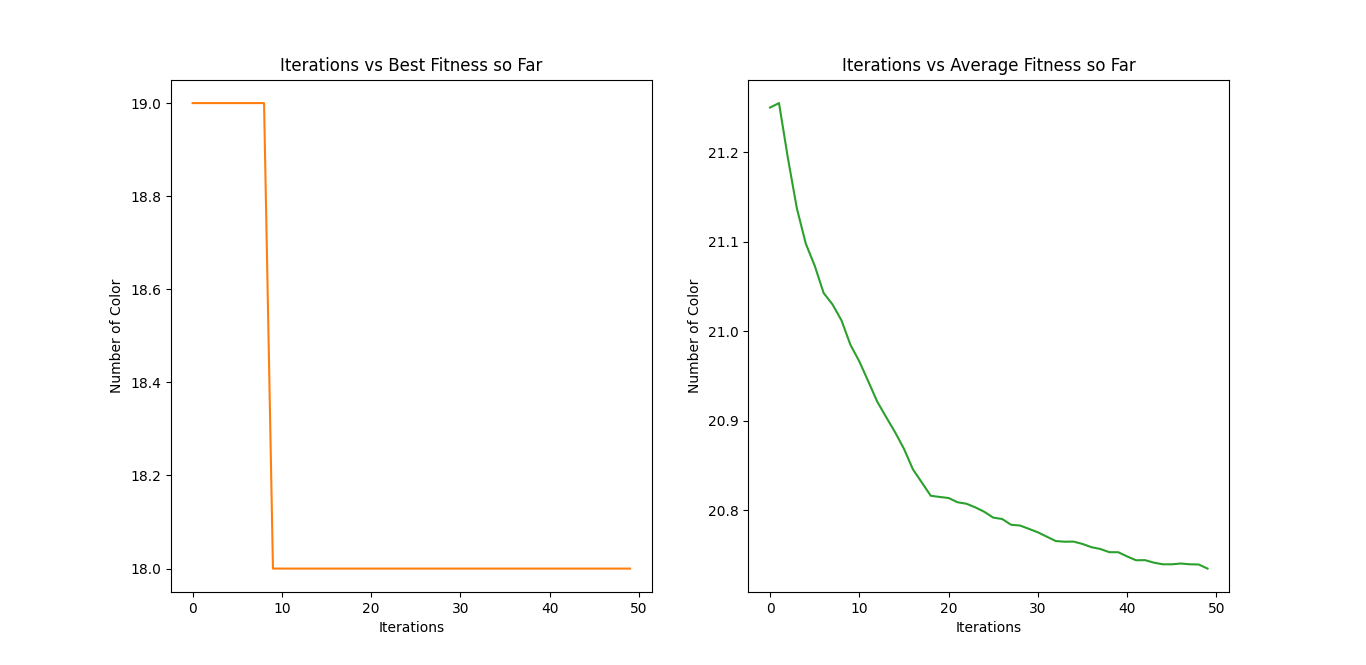
\includegraphics[width=12cm]{Figures/fig7.png}
    \caption{Influence of $\alpha = 1$ on the perfomance of ANTCOL algorithim}
    \end{figure}
\end{center}
When we decrease the value of $\alpha=1$, the quality of the optimal solution also decreased. Ants follow the path which has a higher pheromone concentration.
In turn, the pheromone concentration increases after the increasing number of ants. Overtime, the solution converges to the shortest path. However, 
decreasing the value of $\alpha$ means there is a less chance of picking a route with high pheremone concentration. The solution obtained does not converge to the shortest path 
and the solution that is obtained is of a lower quality.
\newpage

\begin{center}
    \begin{figure}[h]
    \centering
    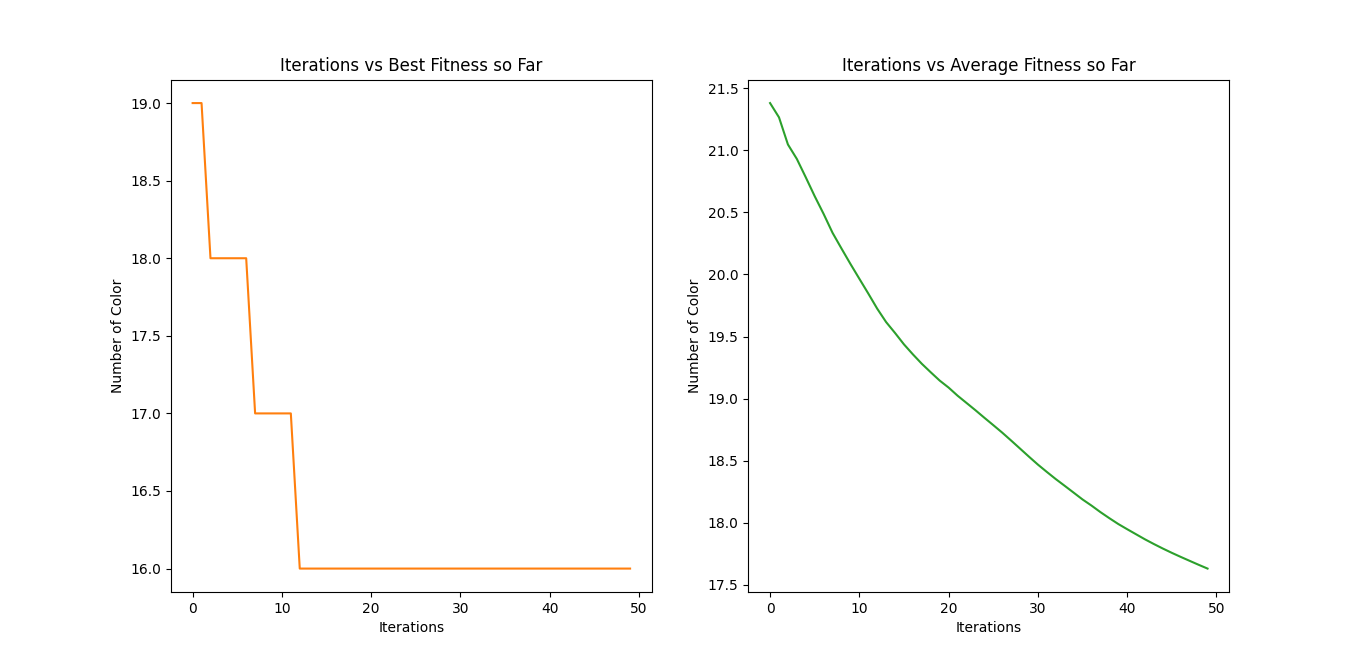
\includegraphics[width=12cm]{Figures/fig8.png}
    \caption{Influence of $\beta = 2$ on the perfomance of ANTCOL algorithim}
    \end{figure}
\end{center}
Decreasing the value of $\beta = 2$ did not have a significant impact on the quality of the coloring that was obtained. This is because the probability of choosing a solution with a higher pheromone concentration is controlled by 
determined by $\alpha$ while $\beta$ determines the desirability of a particular solution. 
\begin{center}
    \begin{figure}[h]
    \centering
    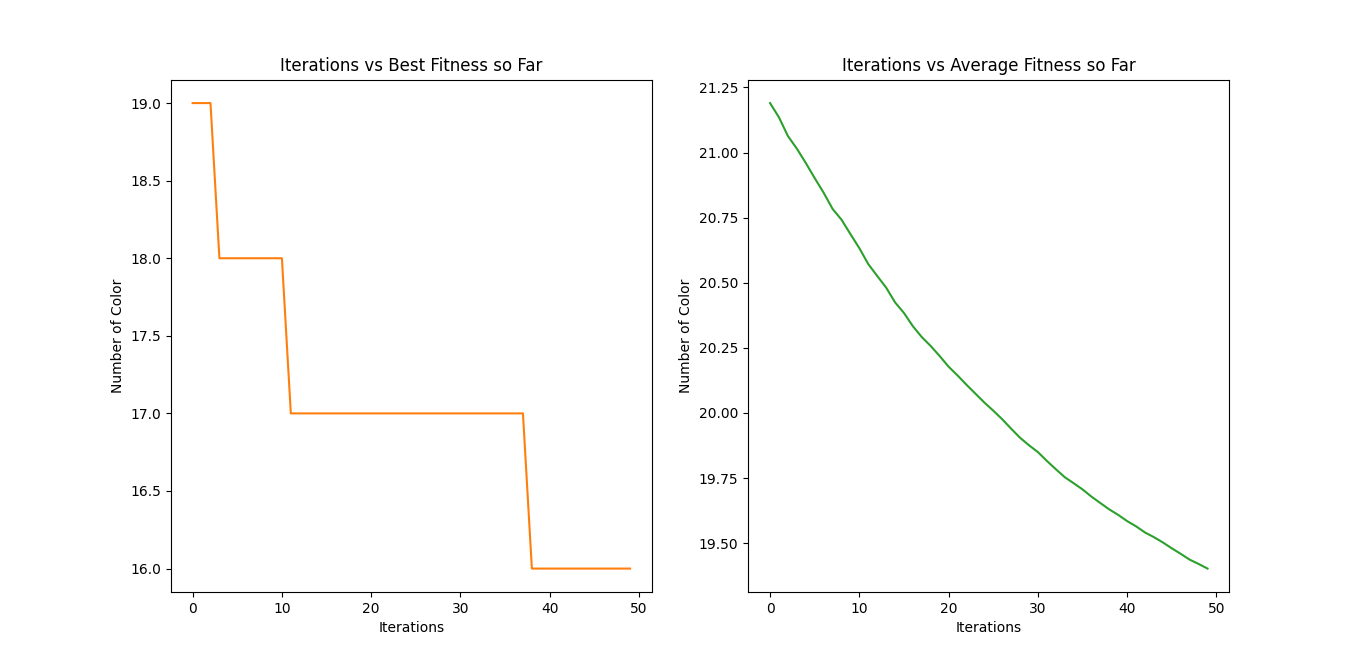
\includegraphics[width=12cm]{Figures/fig9.png}
    \caption{Influence of $\rho = 0.1$ on the perfomance of ANTCOL algorithim}
    \end{figure}
\end{center}

Decreasing the value of $\rho = 0.1$ had a negeligble impact on the quality of the solutions that were obtained but the average quality of the solutions that were obtained greatly decreased. This because a higher concentration of pheremone can lead to risk of being stuck in the local optima.
Decreasing the evaporation rate, means that pheremone concentration is builds up at a faster rate and ants follow the router which has a higher concentration of pheremone. 

\newpage

\begin{center}
    \begin{figure}[h]
    \centering
    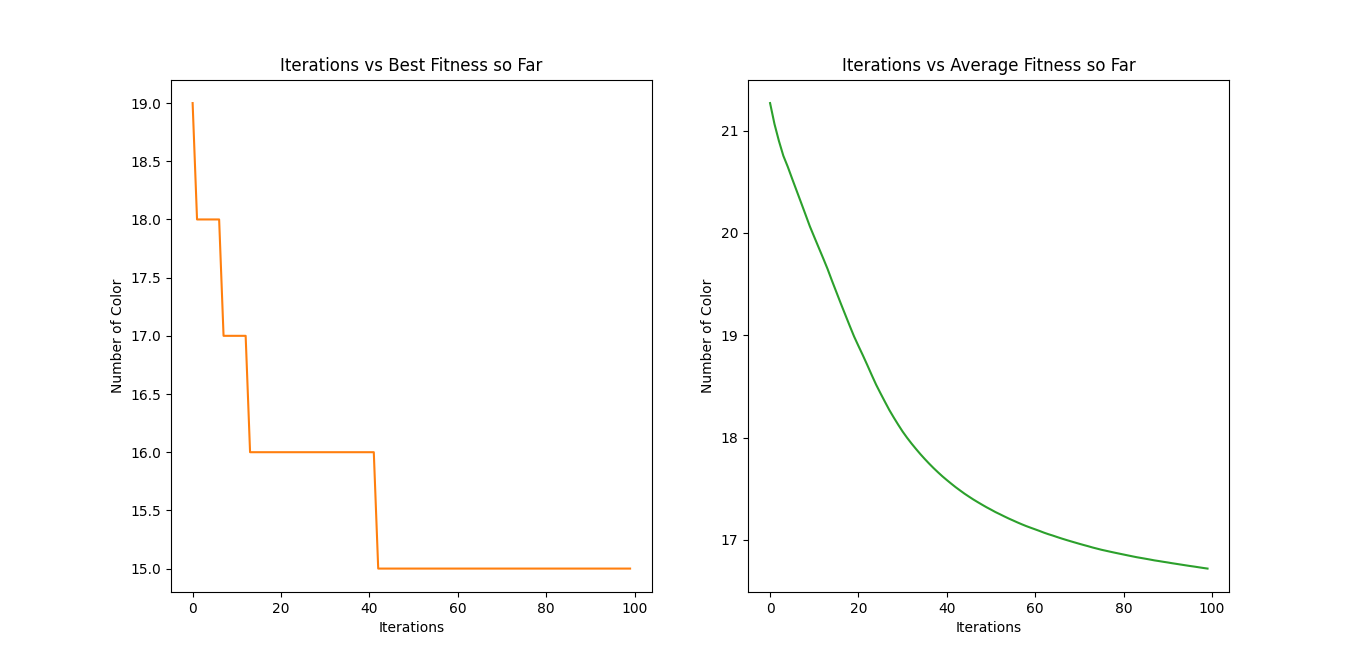
\includegraphics[width=12cm]{Figures/fig10.png}
    \caption{Influence of $N_{cycles} = 100$ on the perfomance of ANTCOL algorithim}
    \end{figure}
\end{center}
Increasing the value of $N_{cycles}=100$ improved the quality of the optimal solution greatly. This because we are using randomization to add the first vertex $v_i$ to the color class $C_k$ and that can result in ineffecient 
exploring of the search space. A suitable number of iterations would allow the search to escape the local optima and converge to the optimal solution.
\begin{center}
    \begin{figure}[h]
    \centering
    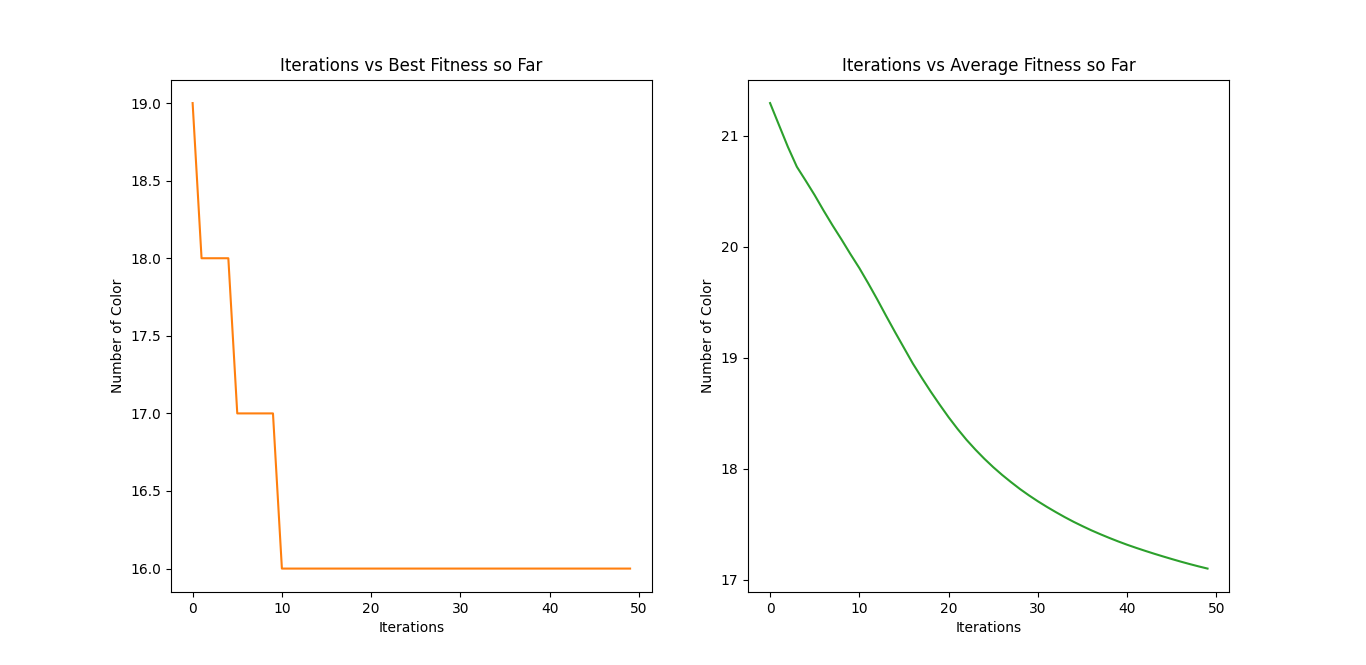
\includegraphics[width=12cm]{Figures/fig11.png}
    \caption{Influence of $N_{ants} = 300$ on the perfomance of ANTCOL algorithim}
    \end{figure}
\end{center}

Although increasing the $N_{ants} = 300$ did not improve the optimal coloring that was obtained the average quality of the solutions that were obtained improved. This is because as increasing number of ants travel through a route
which has high pheremone concentration, the obtained solution will converge to the optimal solution faster i.e 10 iterations instead of about 15 iterations. One downside of increasing the number of ants is that the time taken to execute
increases linearly with the size of ant colony.
\newpage
\begin{center}
    \begin{figure}[h]
    \centering
    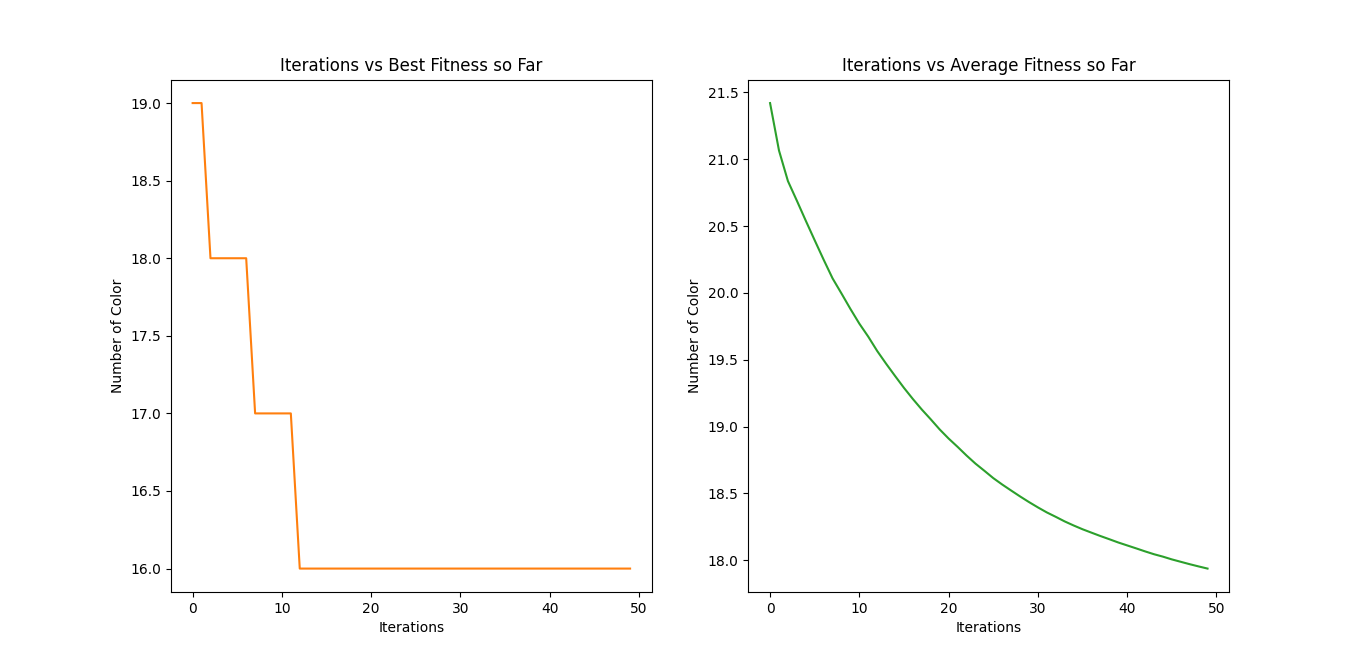
\includegraphics[width=12cm]{Figures/fig12.png}
    \caption{Influence of $Q = 10$ on the perfomance of ANTCOL algorithim}
    \end{figure}
\end{center}
Increasing the value of $Q=10$ didn't have a significant affect on the quality of the colorings that were obtained. This is because $Q$ is a constant and acts as a scaling constant
of the pheromone trail values. 
\section*{Conclusion}

Based on the results, we saw that using a random strategy to choose the first vertex led to diverse solutions and prevented the search from being stuck in a local optima. Furthermore, the trail factor
plays an essential role in the quality of the results that were obtained. Moreover, we saw that a larger colony of ants meant a tradeoff between the rate of convergence to a optimal solution and the running time
of the algorithim. Another factor that played a huge role in improving the quality of solutions was the number of cycles. Fewer cycles could lead to the solution not convreging an on the other hand larger number of
cycles could lead to uneccessary exploration in the search space. The value of $\rho =0.5$ is appropriate as decreasing the evaporation rate can lead to premature convergence.

\newpage
\begin{thebibliography}{2}

    \bibitem{aa} E. Salari and K. Eshghi, ``An ACO algorithm for graph coloring problem,''\textit{2005 ICSC Congress on Computational Intelligence Methods and Applications}, Istanbul, Turkey, 2005, pp. 5 pp.-, doi: 10.1109/CIMA.2005.1662331.
    
    \bibitem{bb} D. Costa and A. Hertz, ``Ants can colour graphs,''\textit{The Journal of the Operational Research Society}, vol. 48, no. 3, p. 295, 1997. 
    
\end{thebibliography}

\end{document}